%!TEX root = ../my_thesis.tex

\appendix

\chapter{Compléments au Chapitre 1}
\section{Détails 1}\label{append:decoding_nodes}

Les sorties du canal composite sont des informations souples données par le démodulateur.
Ce bruit additif est ajouté à la valeur des données en sortie du modulateur $\mathbold{x}$.
\begin{equation}
y_i = x_i + n_i
\end{equation}
Dans le modèle de chaine de communication considéré, la puissance du bruit du canal AWGN $N_0$ est supposée connue.
Cela permet au démodulateur de calculer la probabilité conditionnelle suivante.
\begin{equation}
	p_i = P_r( \tilde{y}_i|\tilde{x}_i) = \frac{1}{\sqrt{\pi N_0}}\exp^{-\frac{(\tilde{x}_i^2-\tilde{y}_i^2)}{N_0}}
\end{equation}
$p_i$ représente la probabilité de recevoir $\tilde{y}_i$ en présupposant la valeur de $\tilde{x}_i$ en sortie du modulateur ($\tilde{x}_i=-1$ ou $\tilde{x}_i=1$).


\textit{likelihood ratio} $L_i$ can be used to represent this information: 
\begin{equation}
	L_i = \dfrac{P_r(y_i | x_i = 0)}{P_r(y_i | x_i = 1)} = \dfrac{p_i}{1 - p_i}
	\label{eq:lr}
\end{equation}
An alternative is the \textit{log-likelihood ratio}
\begin{equation}
	\lambda_i = log(L_i);
	\label{eq:llr}
\end{equation}

Block error correction codes can be defined by a set of parity constraints. This set of constraints can be represented graphically by a tanner graph including equality nodes and parity check nodes. A parity check node is represented in Figure \ref{fig:parite}.

\begin{figure}[t]
\centering
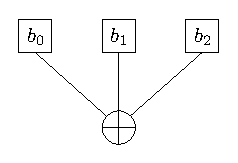
\includegraphics{tail/appendix_1_fig/parite3}
\caption{Parity check node}
\label{fig:parite}
\end{figure}

Equivalently, this can be written as the following parity equation:
\begin{equation}
b_0 + b_1 + b_2 = 0
\end{equation}

The encoder maps a random K-bits vector to a codeword that satisfies the parity constraints of the code. Then the codeword is modulated and sent through the communication channel. On the receiver side, the channel information of each bit is used as an input for the decoder.
The belief propagation decoding process consists in combining information from the channel with the code constraints in order to take a decision on each bit value. In the example of Figure \ref{fig:parite}, the channel estimations of $b_1$ and $b_2$ can be combined with the parity constraints in order to calculate a estimation of $b_0$.

As the estimation of $b_0$ does not use the estimation coming from the channel $L_0$, the notation $L^e_0$ is used, with $e$ for \textit{extrinsic}.
From (\ref{eq:lr}),
\begin{equation}
L^e_0 = \dfrac{P(y_1,y_2 | b_0 = 0)}{P(y_1,y_2 | b_0 = 1)}
\label{eq:le0}
\end{equation}
Only two combinations of $b_1$ and $b_2$ imply that $b_0=0$, that is $b_1=0$, $b_2=0$ or $b_1=1$ and $b_2=1$. One can then calculate $P(b_0|y_1,y_2)$.
\begin{eqnarray}
\begin{array} {r c l}
P(y_1,y_2 | b_0 = 0) & = & P(y_1 | b_1 = 0)P(y_2 | b_2 = 0) + P(y_1 | b_1 = 1)P(y_2 | b_2 = 1)\\
\label{eq:b0y1y2full}
& = &  p_1p_2 + (1-p_1)(1-p_2)
\end{array}
\label{eq:b0y1y2}
\end{eqnarray}
Similarly,
\begin{eqnarray}
\begin{array} {r c l}
P(b_0 = 1 | y_1,y_2) =  p_1(1-p_2) + (1-p_1)p_2
\label{eq:b1y1y2}
\end{array}
\end{eqnarray}

We can deduce from (\ref{eq:le0}), (\ref{eq:b0y1y2}) and (\ref{eq:b1y1y2}) : 
\begin{eqnarray*}
\begin{array} {r c l}
L^e_0 & = & \dfrac{p_1p_2 + (1-p_1)(1-p_2)}{p_1(1-p_2) + (1-p_1)p_2} \\
& = & \dfrac{1 + \dfrac{p_1}{(1-p_1)}\dfrac{p_2}{(1-p_2)}}{\dfrac{p_1}{(1-p_1)}+\dfrac{p_2}{(1-p_2)}} 
\end{array}
\end{eqnarray*}

\begin{equation}
L^e_0=\dfrac{1 + L_1L_2}{L_1+L_2}
\label{eq:parity}
\end{equation}

The other node is the equality node, represented in Figure \ref{fig:equality}.

\begin{figure}[t]
\centering
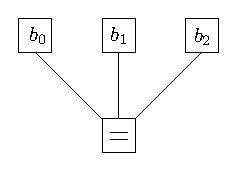
\includegraphics{tail/appendix_1_fig/equality}
\caption{Equality node}
\label{fig:equality}
\end{figure}

Expressing the fact that the only possibility to have $b_0=0$ is that $b_1 = b_2 = 0$ and that the only possibility to have $b_0=1$ is that $b_1=b_2=1$, we can state that:
\begin{eqnarray*}
\begin{array}{r c c c l}
P(y_1,y_2|b_0=0) & = & P(y_1|b_1=0) P(y_2 | b_2 = 0) & = & p_1p_2 \\
P(b_0=1|y_1,y_2) & = & P(y_1|b_1=1) P(y_2 | b_2 = 1) & = & (1-p_1)(1-p_2)
\end{array}
\end{eqnarray*}
We can then deduce the extrinsic:
\begin{equation*}
L^e_0=\dfrac{p_1}{(1-p_1)}\dfrac{p_2}{(1-p_2)}
\end{equation*}
\begin{equation}
L^e_0=L_1L_2
\label{eq:equality}
\end{equation}

SC decoding of polar code can be seen as an instance of BP decoding with a particular scheduling and decision making.

\subsubsection{Successive Cancellation Decoding}
SC decoding sequentially use the equations  (\ref{eq:parity}) and (\ref{eq:equality}) to decode the polar code graph.
There are two levels of decoding: \textit{soft estimations} and \textit{hard decisions}. Soft decisions are mathematically represented by probabilities, likelihood ratios or log-likelihood ratios. In our examples and to use the former equations, likelihood ratios will represent soft estimation. The hard decisions are classically called partial sums and are mathematically represented by values in $\{0,1\}$ and are noted $S_{i,j}$ where $i$ represents the lane, and $j$ represents the stage (also called depth) of the partial sum in the factor graph. Same indexes notations are used for other objects in the graph. The introduction of these notations along with equality nodes will enrich the representation of the factor graph. The following figures represent the different decoding steps for a polar code of size $N=2$.

\begin{figure}[!ht]
  \centering
  \subfloat[][Channel LRs]{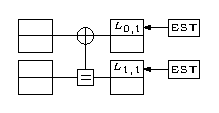
\includegraphics[width=.35\textwidth]{tail/appendix_1_fig/SC_graph2_a}}\quad
  \subfloat[][$F$ function]{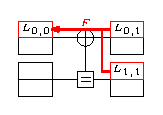
\includegraphics[width=.24\textwidth]{tail/appendix_1_fig/SC_graph2_b}}\quad
  \subfloat[][$H$ function]{
\includegraphics[width=.29\textwidth]{tail/appendix_1_fig/SC_graph2_c}}\\
  \subfloat[][$G$ function]{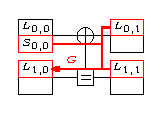
\includegraphics[width=.25\textwidth]{tail/appendix_1_fig/SC_graph2_d}}\quad
  \subfloat[][$H$ function]{
\includegraphics[width=.29\textwidth]{tail/appendix_1_fig/SC_graph2_e}}\quad
  \subfloat[][$H_u$ and $H_l$ functions]{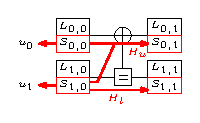
\includegraphics[width=.32\textwidth]{tail/appendix_1_fig/SC_graph2_f}}
  \caption{Successive Cancellation Scheduling}
  \label{fig:SCSchedule}
\end{figure}

Figure \ref{fig:SCSchedule} shows the sequence of the different operations of successive cancellation decoding algorithm:
\begin{itemize}
\item[(a)] The first step is the loading of the channel likelihood ratios into the decoding factor graph.
\item[(b)] The second step is the computation of the value of $L_{0,1}$. The function used is the computation of the extrinsic of a parity node as described in equation \ref{eq:parity}:
\begin{equation}
L_{0,0} = F(L_{0,1}, L_{1,1}) = \dfrac{1+L_{0,1}L_{1,1}}{L_{0,1}+L_{1,1}}
\end{equation}
\item[(c)] The third step is an hard decision to deduce $S_{0,0}$ from $L_{0,0}$:
 \[
    S_{0,0}=HD(L_{0,0})=
    	\begin{cases} 
    		0 & \text{if }L_{0,0}\geq0.5\\
    		1 & \text{if }L_{0,0}<0.5
    		\end{cases}
  \]
\item[(d)] The fourth step is the computation of the value of $L_{1,1}$. The inputs used are $S_{0,0}$, $L_{0,1}$ and $L_{1,1}$. We see that the equality node is used, so we will use the equality node equation (\ref{eq:equality}). The first member of the equation is $L_{1,1}$. The second member depends on the value of $S_{0,0}$.

\[
	L_{1,0} = 
	\begin{cases} 
	L_{1,1}L_{0,1} & \text{if }S_{0,0} = 0\\
	L_{1,1}\dfrac{1}{L_{0,1}} & \text{if }S_{0,0} = 1
	\end{cases}
\]

This can be simplified:
\begin{equation}
L_{1,0} = G(L_{1,1},L_{0,1},S_{0,0}) = L_{1,1}L_{0,1}^{1 - 2S_{0,0}}
\end{equation}
\item[(e)] Fifth step is an hard decision: 
\begin{equation*}
S_{1,0}=HD(L_{1,0})
\end{equation*}
\item[(f)] Final step is the propagation of the partial sums, which is equivalent to a polar encoder.
\begin{equation}
S_{0,1} = H_u(S_{0,0},S_{1,0}) =S_{0,0}\oplus S_{1,0}
\end{equation}	
\begin{equation}
S_{1,1} = H_l(S_{1,0}) = S_{1,0}\\
\end{equation}

	
\end{itemize}

\chapter{Compléments au Chapitre 2}\label{sec:annCCSDS}
\chapter{Compléments au Chapitre 3}\label{sec:ann3}
